\documentclass[a4paper,12pt]{report}

\usepackage{alltt, fancyvrb, url}
\usepackage{graphicx}
\usepackage{a4wide}
\usepackage[utf8]{inputenc}
\usepackage{hyperref}
\usepackage{float}
\usepackage{listings}
\usepackage[htt]{hyphenat}
% fixa uno warning
\hypersetup{final}

% serve per mandare a capo gli URL troppo lunghi
% non chiedetemi come però 
\usepackage{url}
\makeatletter
\g@addto@macro{\UrlBreaks}{\UrlOrds}
\makeatother

% Questo commentalo se vuoi scrivere in inglese.
\usepackage[utf8]{inputenc}
\usepackage[italian]{babel}
\usepackage[T1]{fontenc}

\usepackage[italian]{cleveref}

\title{\textbf{TRACCIA 1 – Progetto IoT}\\Relazione di progetto\\Programmazione di Reti}

\author{
Stefano Scolari 0000915930 \\
Kelvin Oluwada Milare Obuneme Olaiya 0000921596
}

\date{\today}


\begin{document}

\maketitle

\tableofcontents

\chapter{Analisi}
\section{Requisiti}
Alcuni device IOT si occupano di raccogliere dati ed effettuare misurazioni concernenti temperatura ed umidità, questo per riuscire a mantenere adeguata l'irrigazione di una coltivazione "smart".\\
Si vuole quindi realizzare un sistema di rete composto da un certo numero di device IOT ed un gateway a cui questi ultimi si possano collegare. Il gateway, quando abbia ricevuto le misurazioni da tutti i device, deve inviare i dati ad un server.
\\
Quando il server ha ricevuto i dati si occuperà di visualizzarne il contenuto.
\\
I dispositivi di cui si vuole tenere traccia sono 4, questi inviano aggiornamenti sui dati giornalieri al gateway una volta ogni 4 ore, per un totale di 6 rilevazioni giornaliere.\\
Come precedentemente accennato, i dati devono tracciare l'ora della rilevazione, la temperatura ed umidità rilevata.

\begin{figure}[H]
    \begin{center}
        \centering
        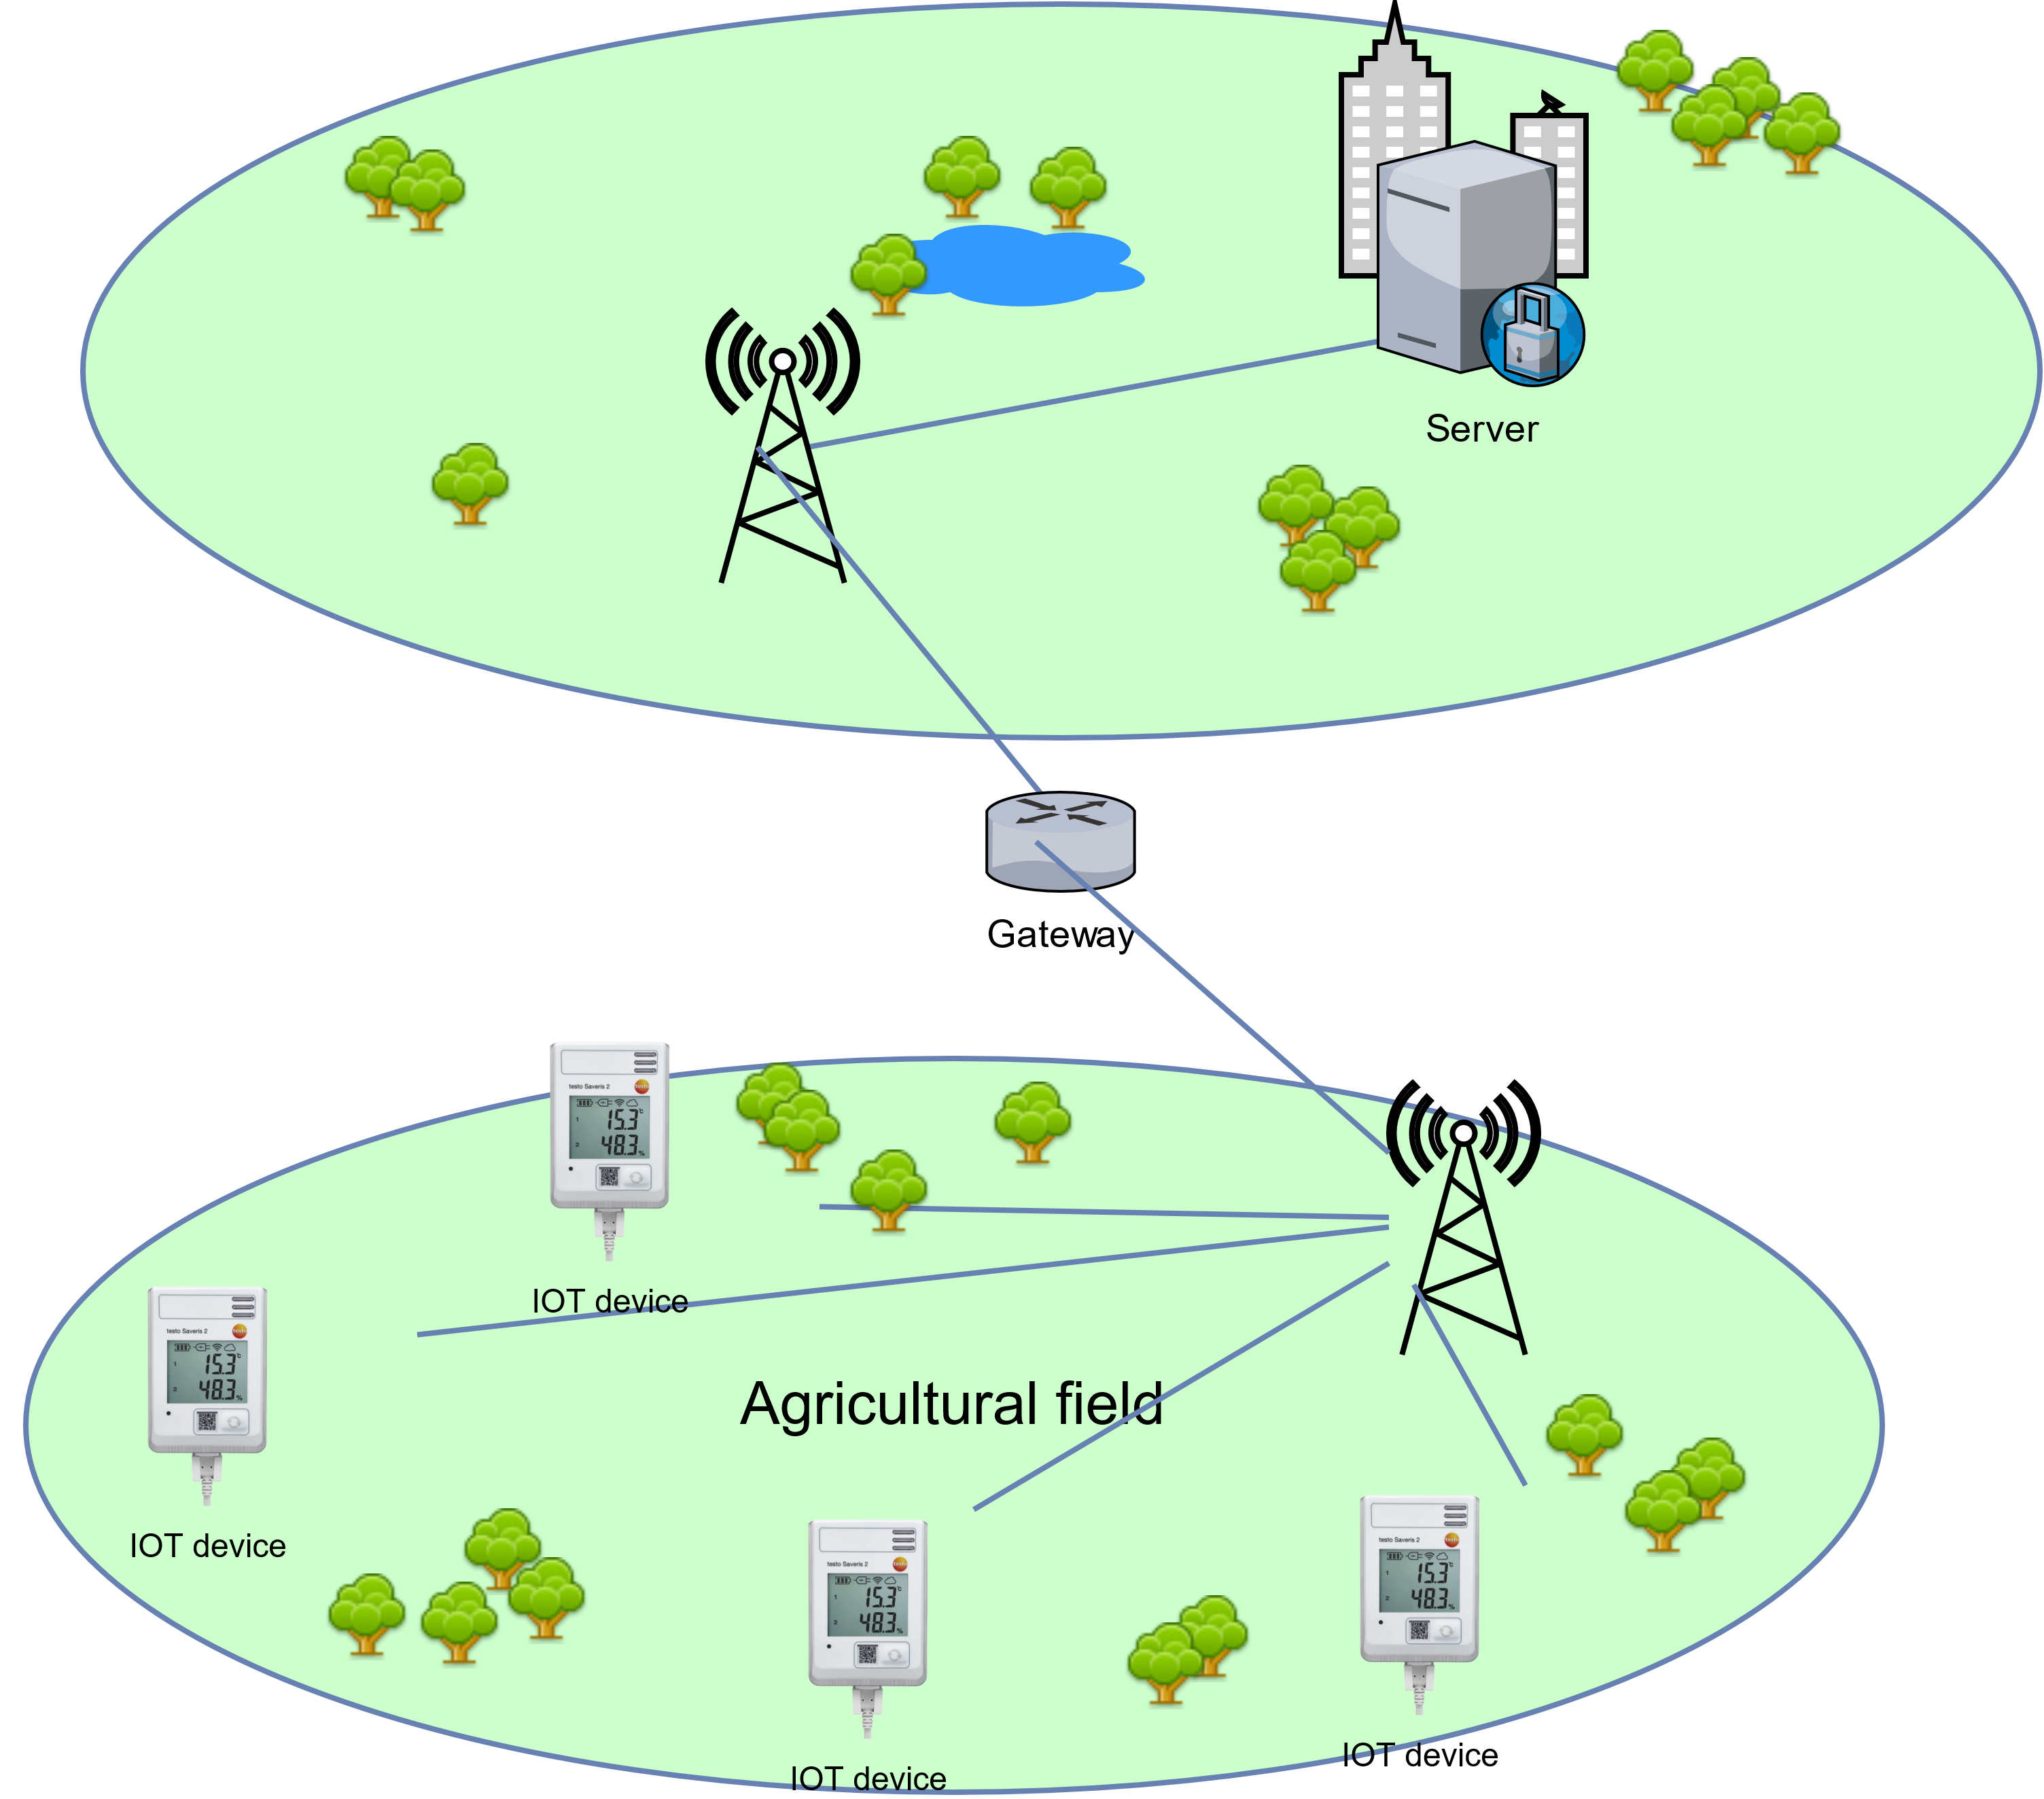
\includegraphics[scale=0.6]{UML/Architecture.png}
    \end{center}
    \caption{Rappresentazione generale della rete}
    \label{img:Architecture}
\end{figure}
\
\\
%

\subsection*{Struttura di rete generale richiesta}
Il commissionante richiede che gli indirizzi IP dei \textbf{Device} IOT appartengano ad una rete di classe C del tipo \texttt{192.168.1.0/24}.\\
Il \textbf{Gateway} deve possedere due interfacce di rete. Una si interfaccia coi dispositivi, appartenente alla loro stessa network. L'altra, che comunica con il \textbf{Server}, ha indirizzo IP appartenente alla classe \texttt{10.10.10.0/24}, a questa stessa classe appartiene anche l'indirizzo IP del server.\\
Si richiede inoltre che i device instaurino connessioni \textbf{UDP} con il Gateway per inviare i dati, mentre si avrà una connessione \textbf{TCP} tra Gateway e Server.

\chapter{Design}

\section{Architettura di Rete}
La \cref{img:ArchitetturaGenerale} mostra l'architettura di rete implementata per realizzare il sistema richiesto.

\begin{figure}[H]
    \begin{center}
        \centering
        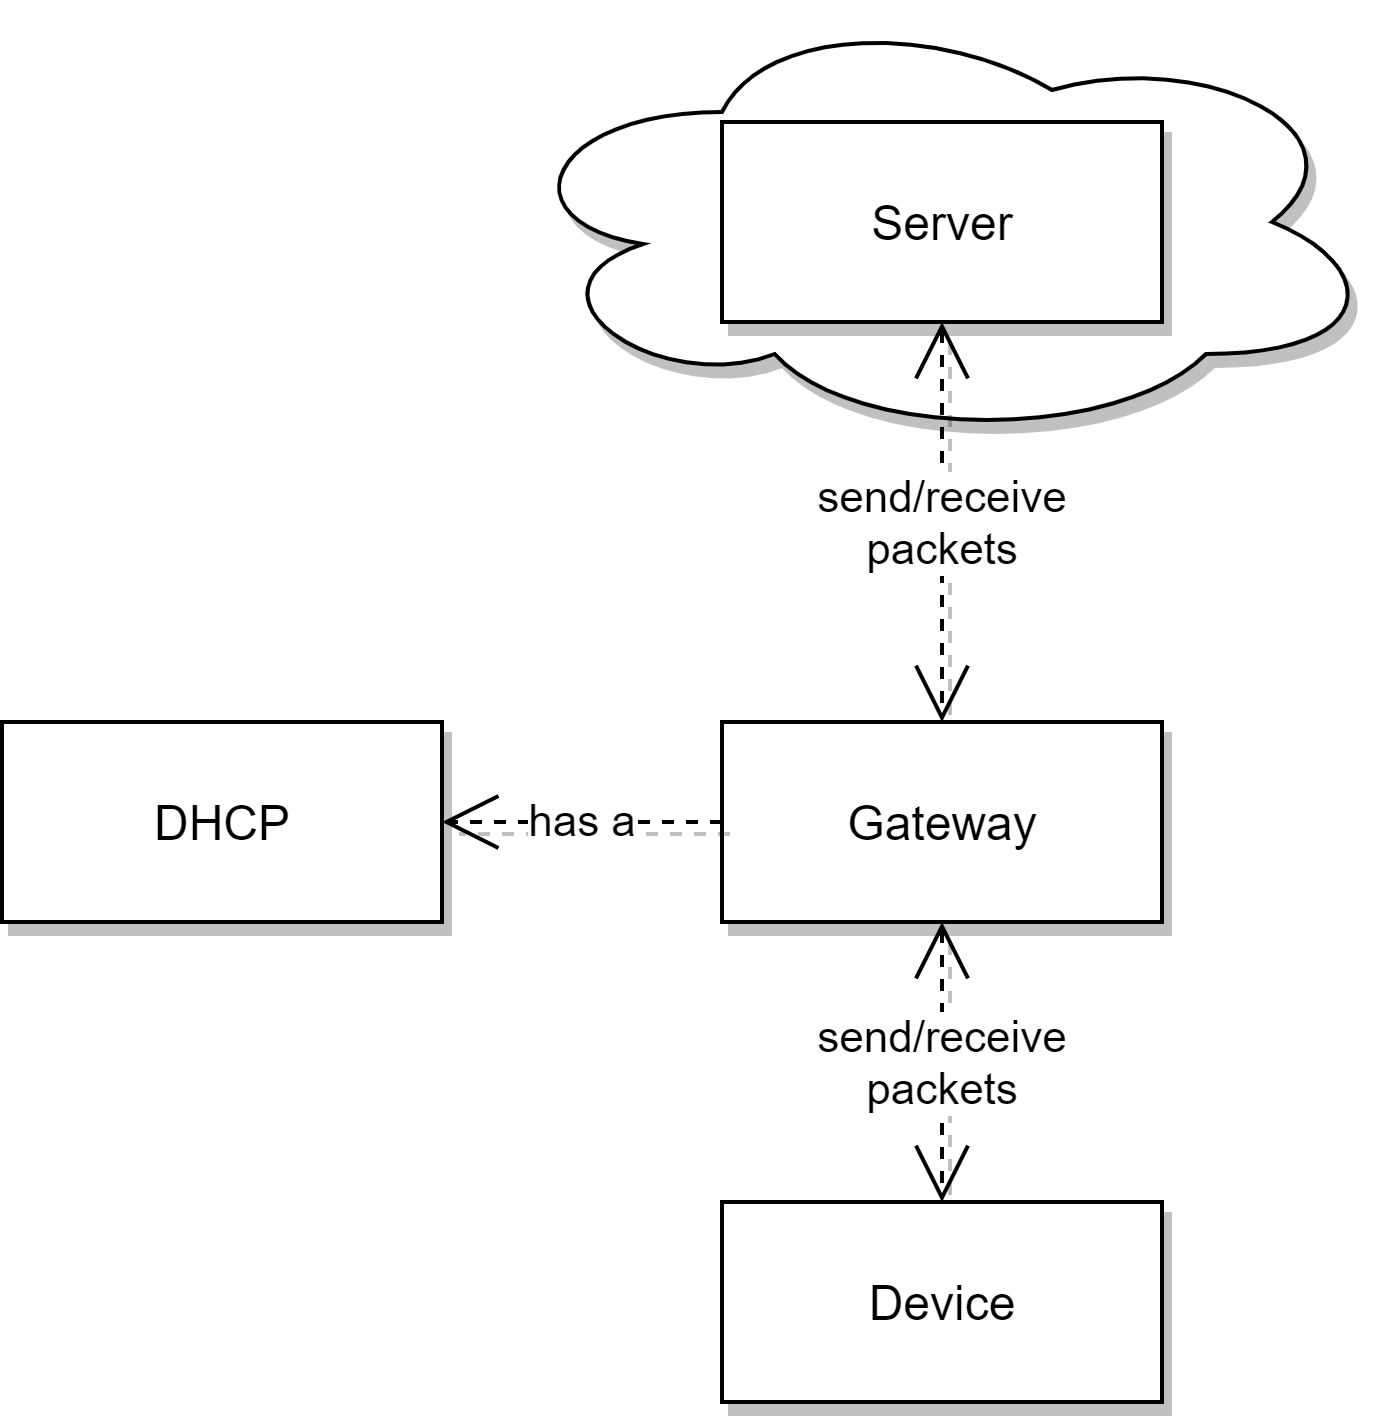
\includegraphics[scale=1]{UML/ArchitetturaGenerale.png}
    \end{center}
    \caption{Schema UML architettura di rete generale}
    \label{img:ArchitetturaGenerale}
\end{figure}
\
\\
%
\subsection*{Device}
I Device, alla loro creazione iniziale, con necessaria assegnazione dell'indirizzio MAC, richiedono automaticamente al server DHCP del Gateway di ricevere un indirizzo IP per la loro sottorete.\\
Quando un dispositivo ha raccolto i dati delle 24h, sempre attraverso una connessione UDP, si occuperà di inviare le misurazioni al Gateway di riferimento.\\
\subsection*{Gateway}
Il Gateway si occupa di raccogliere i dati inviati dai vari dispositivi per mezzo di una connessione UDP.\\
Quando raccolte le misurazioni da parte dei 4 dispositivi, il Gateway deve occuparsi di instaurare una connessione TCP con il Server a cui vuole inviare i dati.
\subsubsection*{DHCP server}
Abbiamo scelto di munire il Gateway di un proprio DHCP, per permettere un'assegnazione automatica degli indirizzi IP della sottorete di cui fanno parte i Device.

\clearpage

\section{Design dettagliato}
Abbiamo scelto di strutturare le varie entità e componenti attraverso la realizzazione di classi, così da poter operare con un'organizzazione di codice maggiormente espressiva e legata alle astrazioni concettuali ideate.

\subsection*{Device}
L'oggetto \textbf{Device} ha il compito di raccogliere le varie misurazioni nell'arco della giornata. Ai fini della simulazione abbiamo deciso di far coincidere la durata di un giorno con il trascorrere di 24 secondi. Ogni 4 secondi verrà quindi aggiunta una nuova misurazione. Trascorsa una giornata verrà instaurata la comunicazione con il gateway per inviare l'elenco delle misurazioni.
\begin{figure}[H]
    \begin{center}
        \centering
        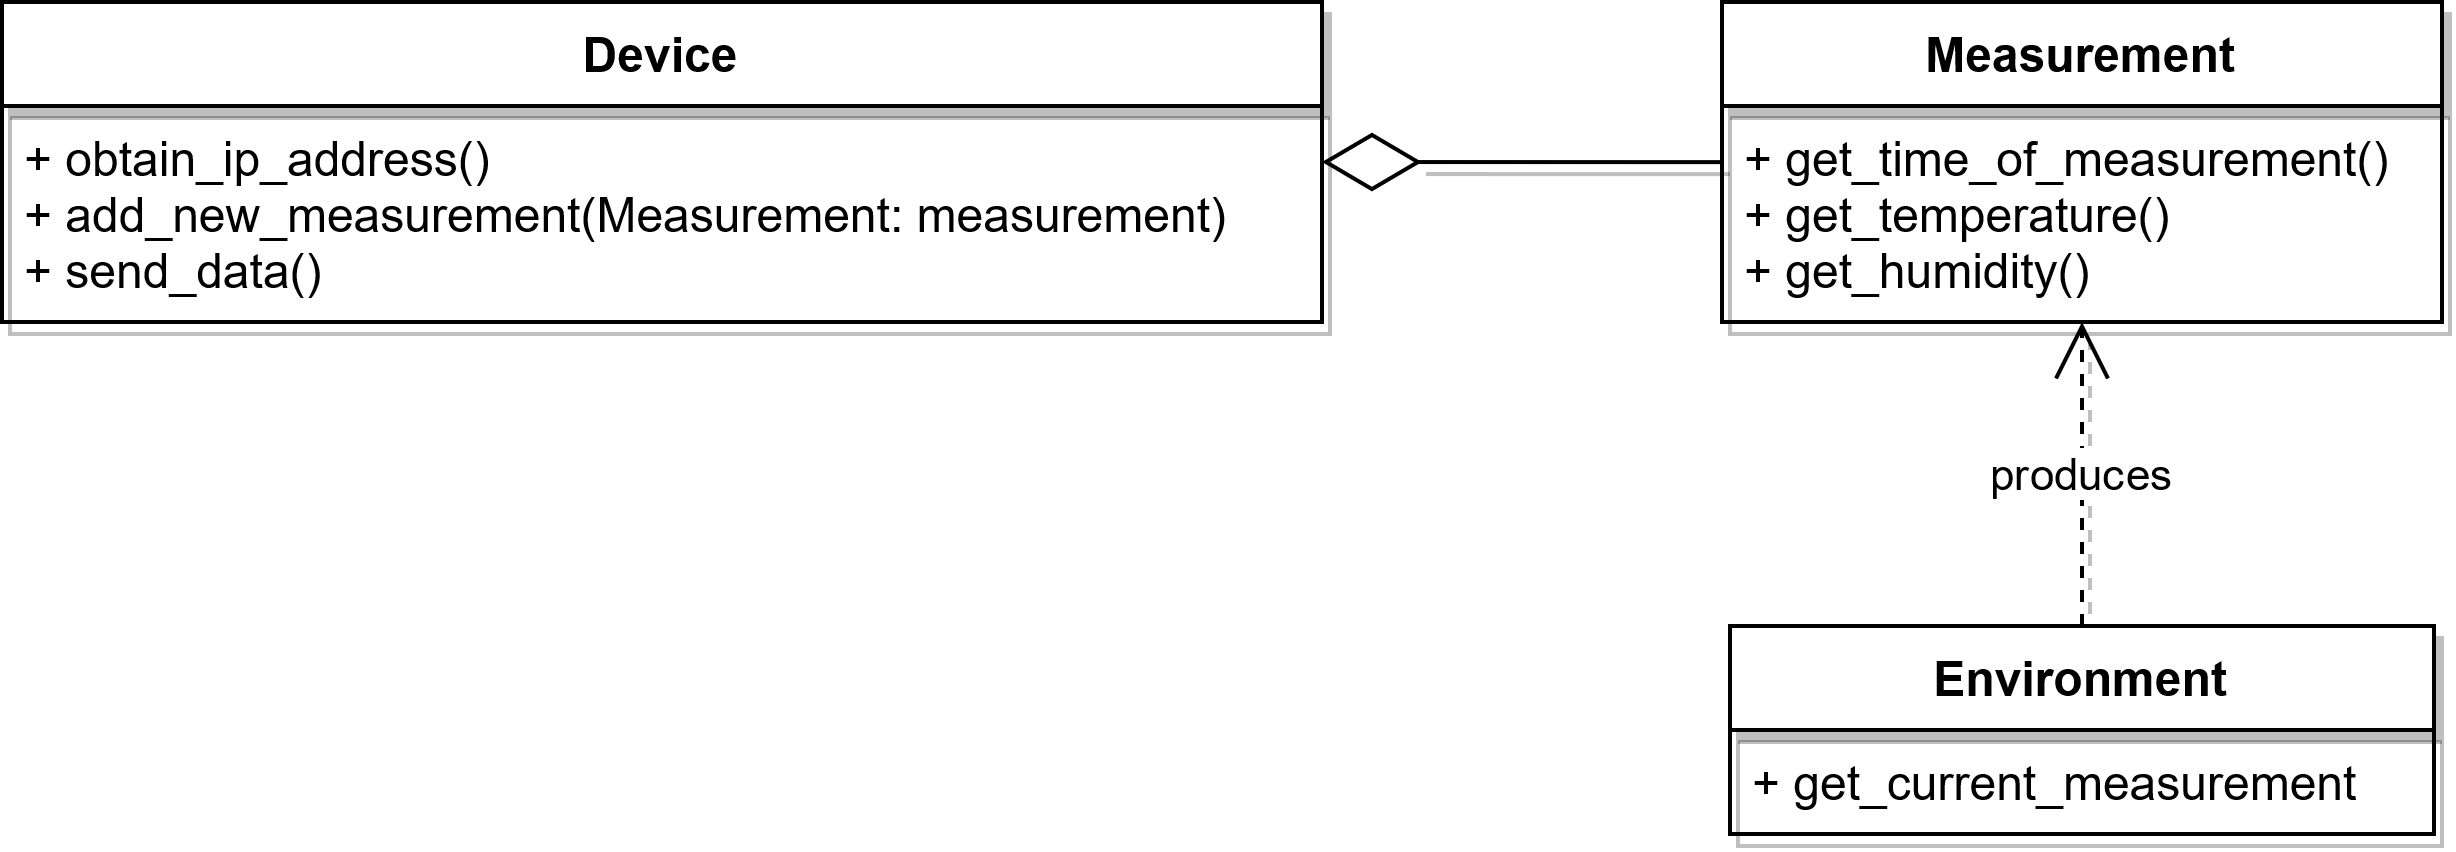
\includegraphics[scale=1]{UML/Device.png}
    \end{center}
    \caption{Device, measurement e environment}
    \label{img:Device}
\end{figure}
\
\\
%
\subsection*{Measurement}
Un oggetto della classe Measurement racchiude dentro di sé i dati relativi all'umidità e temperatura ed inoltre un timestamp di quando quella misurazione è stata acquisita.

\subsection*{Environment}
Per rappresentare a livello astratto dove vengono effettuate le misurazioni, abbiamo scelto di creare una semplice classe Environment, che nel nostro caso, per semplicità, produce i dati in maniera casuale.

\subsection*{Packet}
Lo scambio di informazione tra le diverse entità avviene per mezzo di pacchetti. Anche in questo caso abbiamo operato una semplificazione. Un pacchetto contiente le principali informazioni utili a formare un \texttt{header Ethernet}, \texttt{header IP} ed infine il \texttt{payload} con l'informazione vera e propria. Un pacchetto, inoltre, contiene anche un timestamp di quando questo è stato generato, in maniera tale che sarà poi eventualmente possibile calcolare i tempi di trasmissione.

\begin{figure}[H]
    \begin{center}
        \centering
        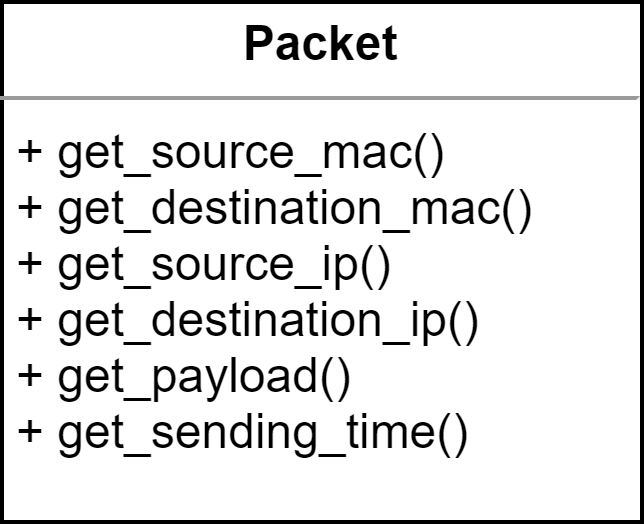
\includegraphics[scale=1]{UML/Packet.png}
    \end{center}
    \caption{Packet}
    \label{img:Packet}
\end{figure}

\subsection*{Gateway}
Il gateway ha il compito di attendere di ricevere le misurazioni da tutti e 4 i dispositivi della rete, per poi successivamente inviarle tutte assieme al server.  
\begin{figure}[H]
    \begin{center}
        \centering
        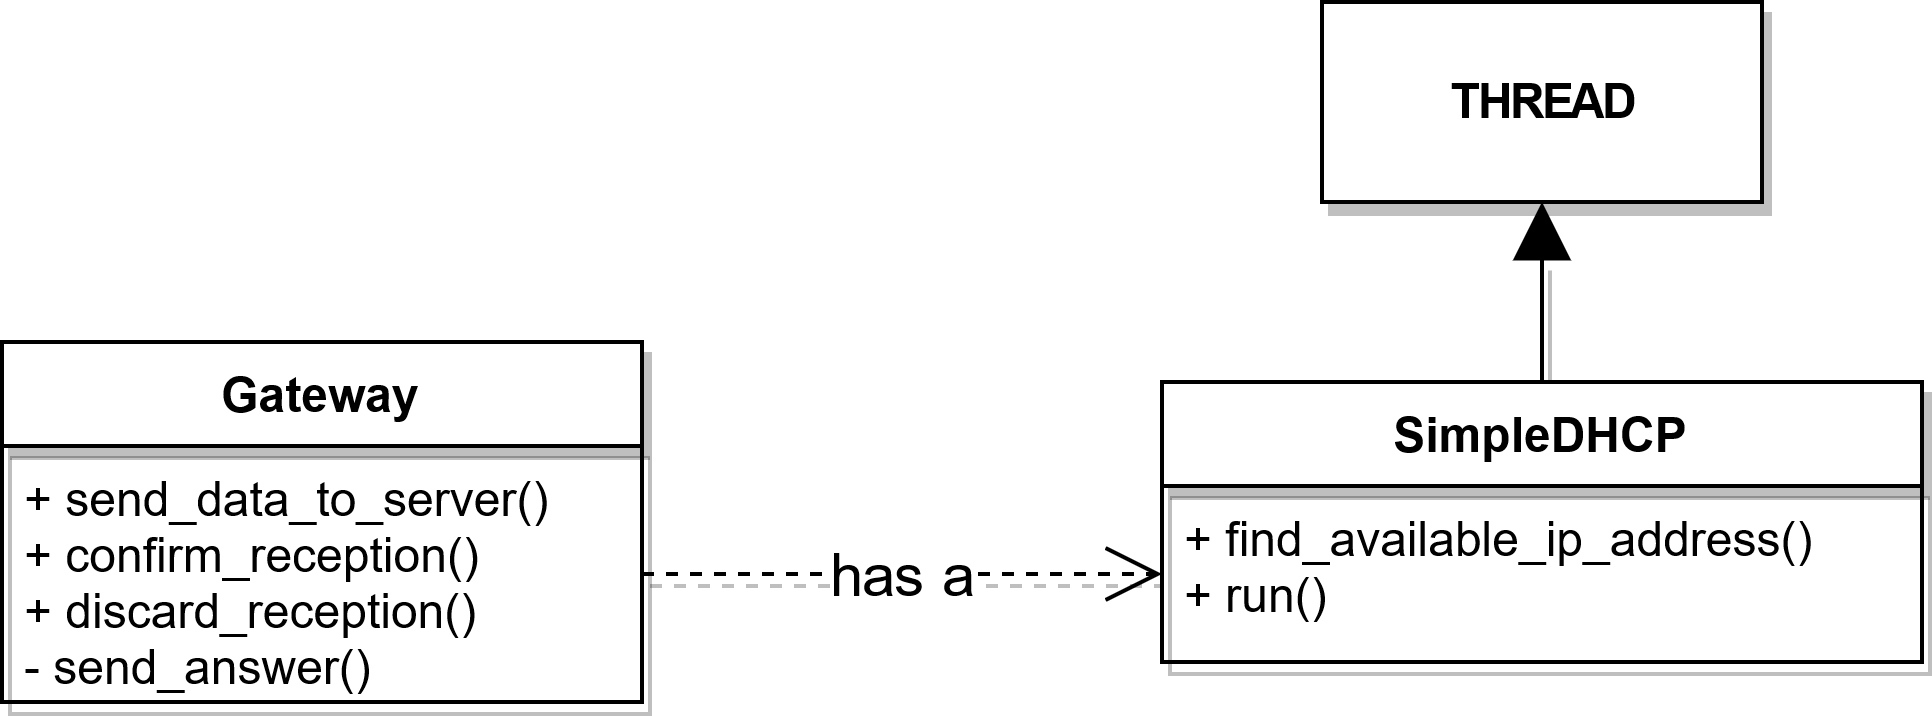
\includegraphics[scale=1]{UML/Gateway.png}
    \end{center}
    \caption{Gateway}
    \label{img:Gateway}
\end{figure}
\
\\
%
\clearpage

\subsection*{DHCP}
Come accennato in precedenza, un device deve essere collegato ad una rete di classe C di tipo \texttt{192.168.1.0/24}. Per far si che ciò avvenga, abbiamo deciso di aggiungere al Gateway un componente DHCP che ha il compito di fornire a chi ne fa richiesta un indirizzo IP appartenente alla suddetta rete.\\
Ai fini della simulazione, il comportamento di questo DHCP risulta semplificato. Il nostro protocollo prevede che il dispositivo faccia una richiesta UDP al DHCP inviando un pacchetto vuoto (Nell'intestazione del pacchetto l'indirizzo IP del mittente sarà \texttt{0.0.0.0}). Quest'ultimo analizzerà l'intestazione del pacchetto estraendone \textit{l'indirizzo MAC}. Se per questo \textit{indirizzo MAC} vi è una corrispondenza nell'\textit{Arp Table} del DHCP, quest'ultimo risponderà al device con un pacchetto che conterrà nel corpo \textit{l'indirizzo IP} che gli è stato precedentemente assegnato. Se invece nell'\textit{Arp Table} non vi è alcuna corrispondenza, l'\textit{indirizzo IP} assegnato avrà un \textit{host number} successivo all'ultimo che è stato concesso nella rete.\\
Come si evince dalla \cref{img:Gateway}, il DHCP è un componente del Gateway, ed abbiamo scelto di renderlo un \texttt{Thread}, in modo da poter operare autonomamente dal Gateway stesso, evitando che DHCP e Gateway effettuino funzionalità bloccanti rispetto all' altro.

\subsection*{Server}
Il ruolo del server è quello di attendere di ricevere le misurazioni dei 4 device e successivamente stamparle a video. 

\section{Schema di comunicazione}
\subsection{Comunicazione Device - DHCP server}
\begin{figure}[H]
    \begin{center}
        \centering
        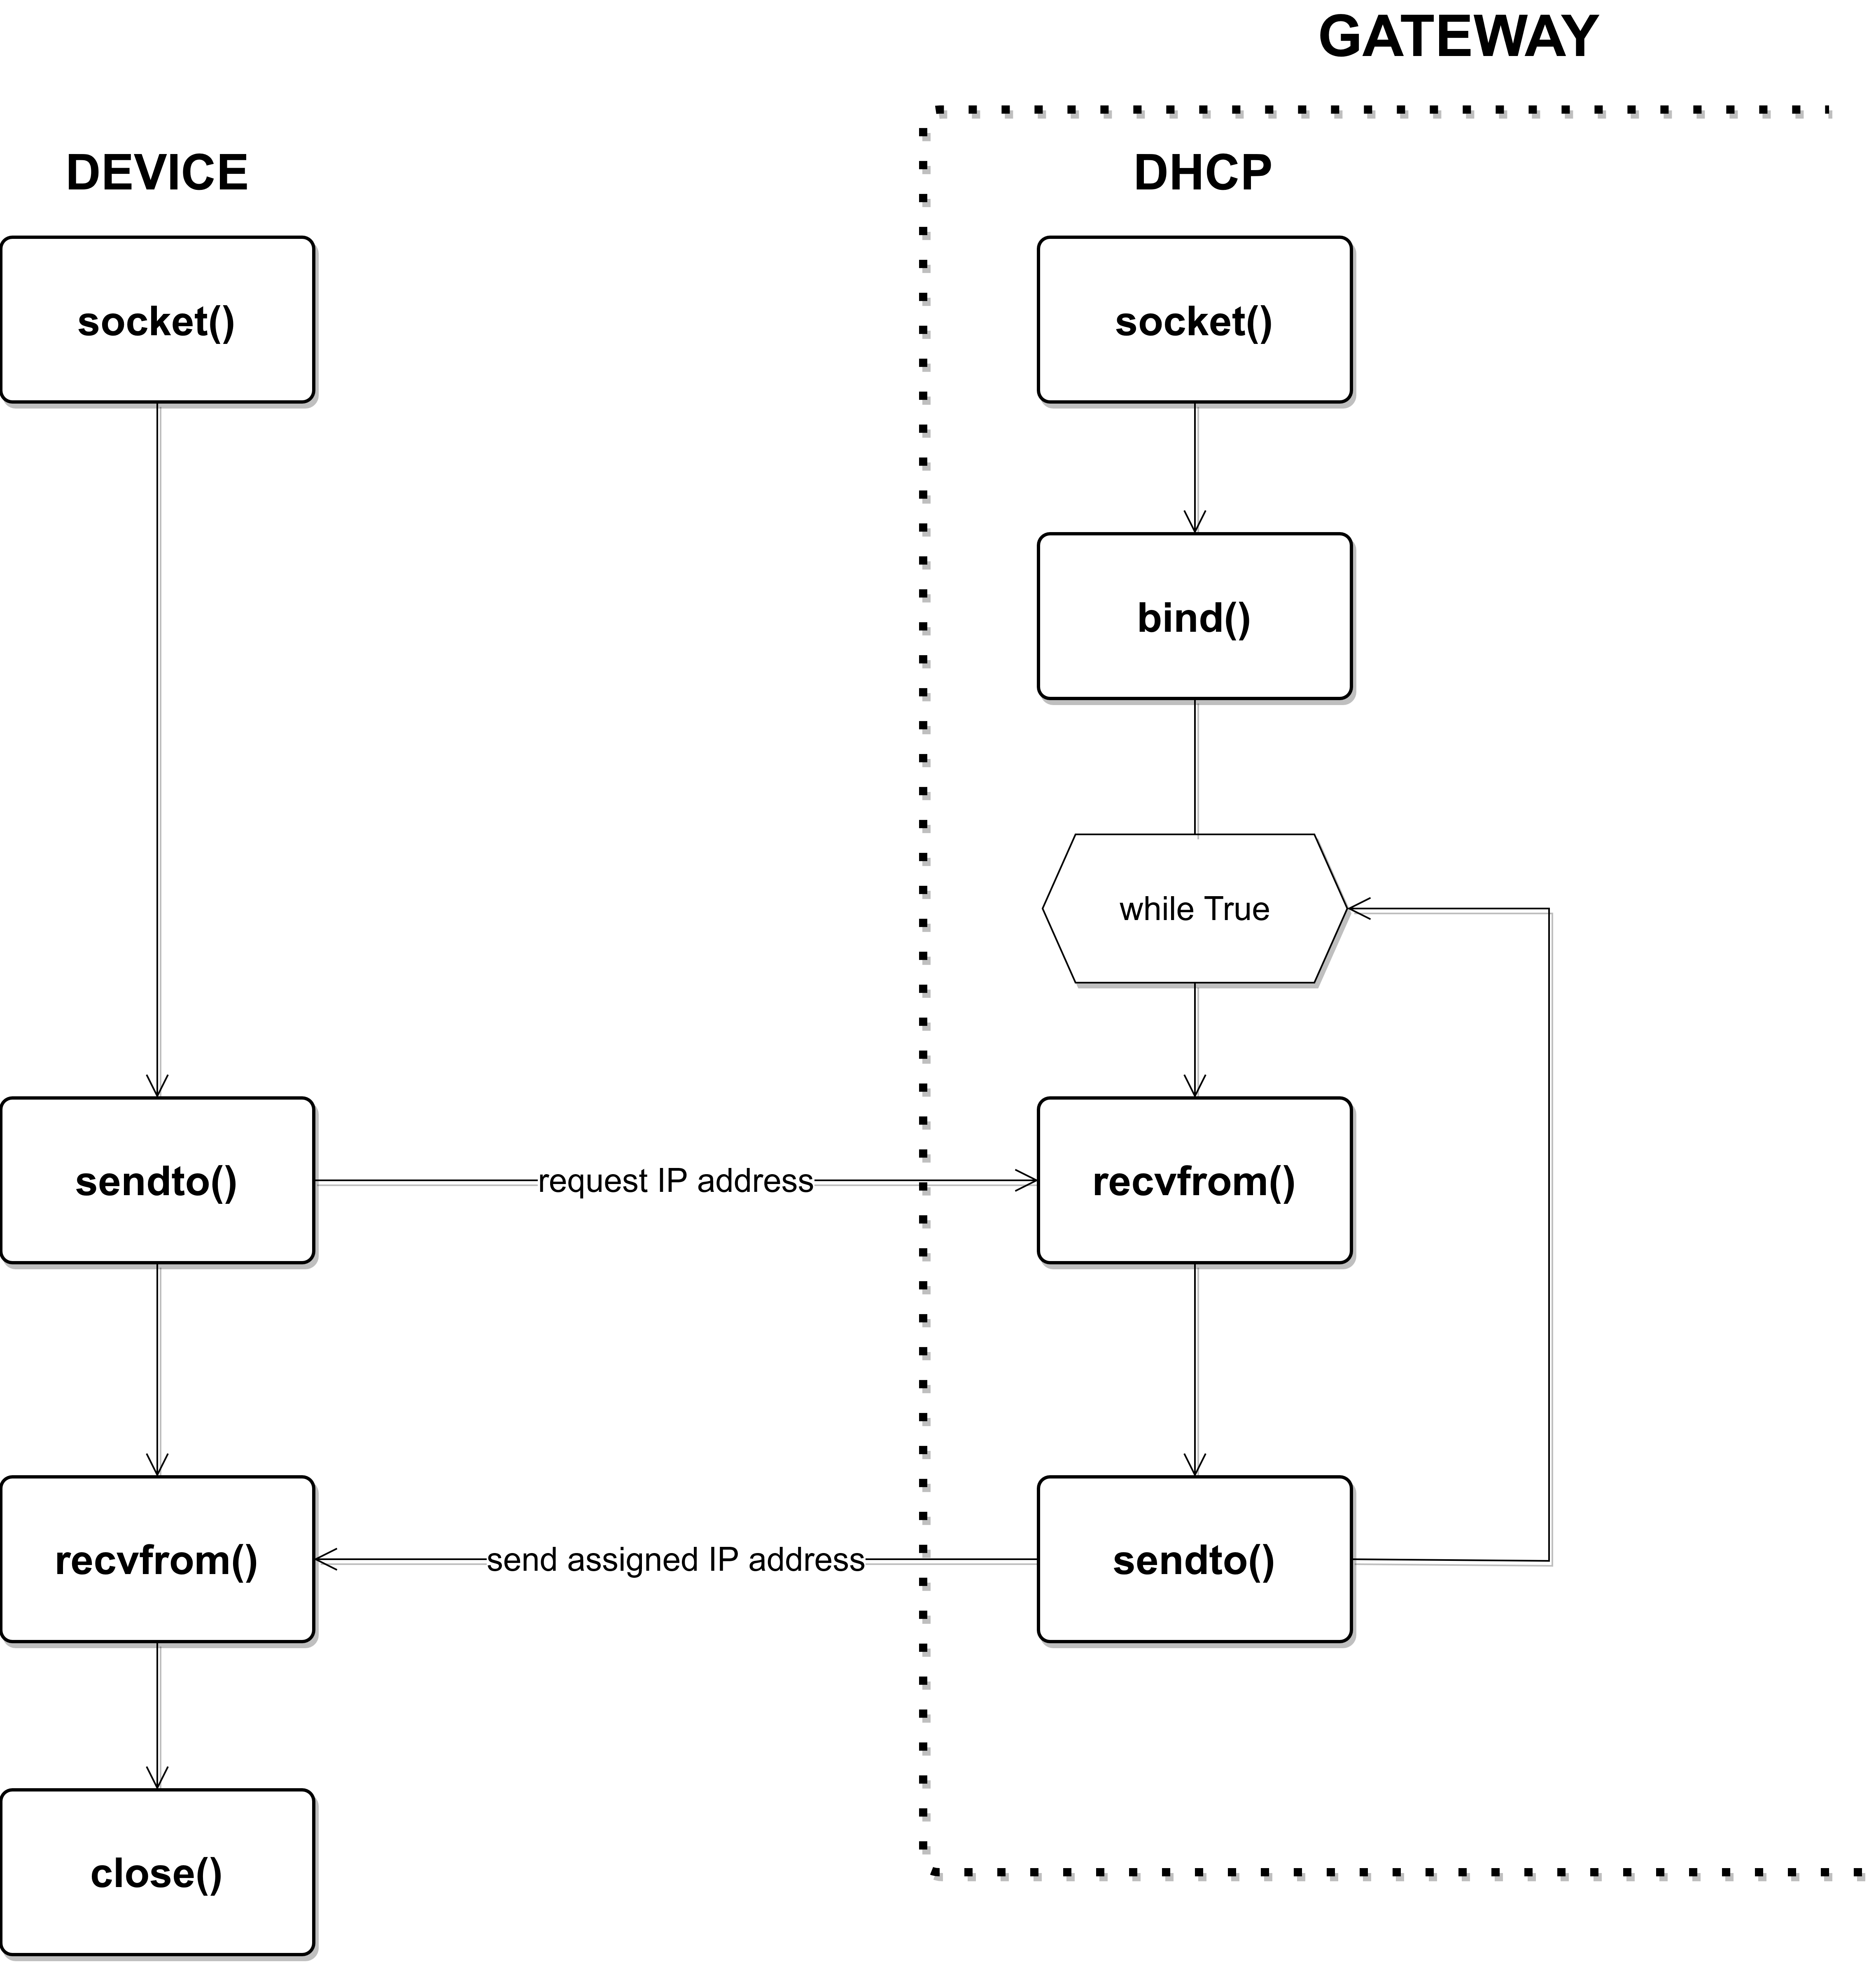
\includegraphics[scale=0.5]{UML/DHCP.png}
    \end{center}
    \caption{Schema rappresentante la comunicazione fra Device e DHCP}
    \label{img:DHCP}
\end{figure}
\
\\
%
\subsection{Comunicazione Device - Gateway}
Dalla \cref{img:DeviceGateway} si può vedere che il device apre una nuova socket \textbf{UDP} ogni volta che intende inviare le proprie rilevazioni al Gateway. \\
Abbiamo optato per questa scelta in modo tale da evitare di tenere impiegate le risorse allocate per mantenere in essere la socket.\\L'invio dei dati non è infatti continuo, e non richiede quindi l'apertura costante della socket.\\ Inoltre, dato che viene utilizzato il \textit{protocollo UDP}, che offre un servizio non affidabile e non orientato alla connessione, abbiamo deciso di far attendere il device per un pacchetto di conferma che dovrà arrivare entro un certo tempo di timeout.\\Nel caso non dovesse pervenire conferma allo scattare del timeout, il device provedderà ad inviare nuovamente le sue misurazioni.\\
In questo modo si cerca di evitare che il Gateway debba aspettare un altro giorno per poter inviare i dati al server.
\begin{figure}[H]
    \begin{center}
        \centering
        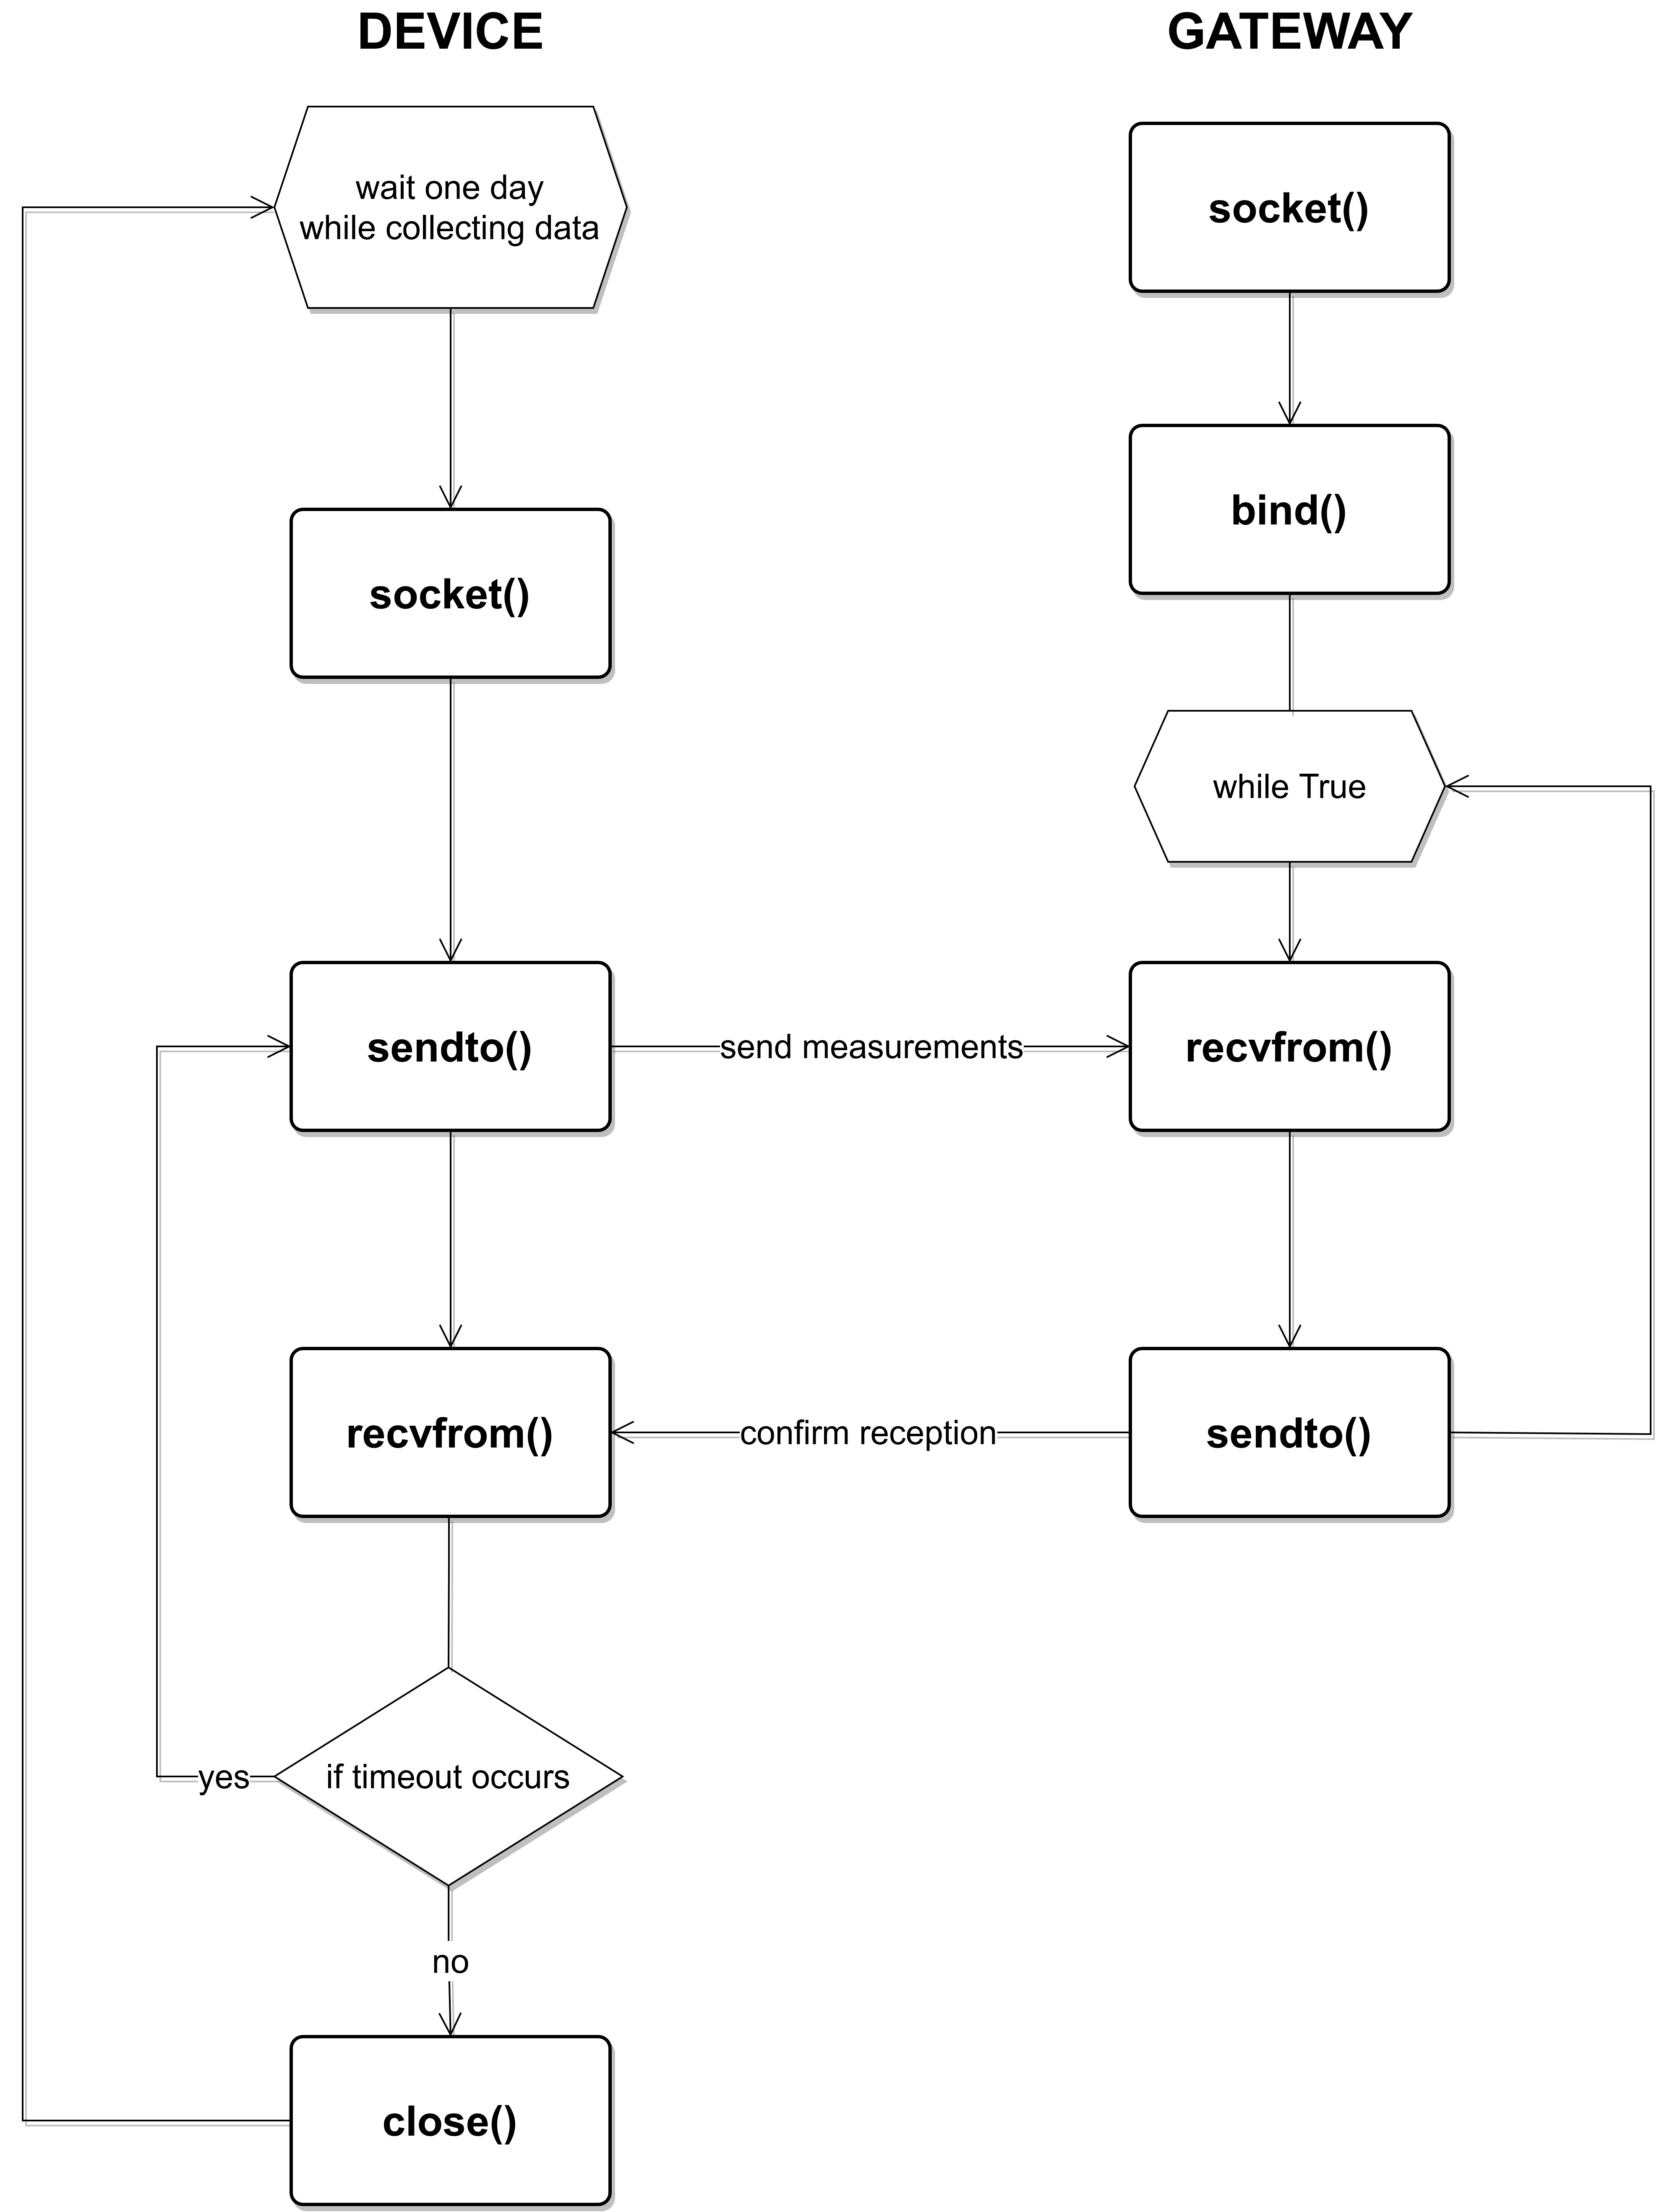
\includegraphics[scale=0.35]{UML/DeviceGateway.png}
    \end{center}
    \caption{Schema rappresentante la comunicazione fra Device e Gateway}
    \label{img:DeviceGateway}
\end{figure}
\
\\
%
\subsection{Comunicazione Gateway - Server}
La creazione della socket \textbf{TCP} avviene solo quando il Gateway ha ricevuto le misurazioni da tutti e 4 i dispositivi.
\begin{figure}[H]
    \begin{center}
        \centering
        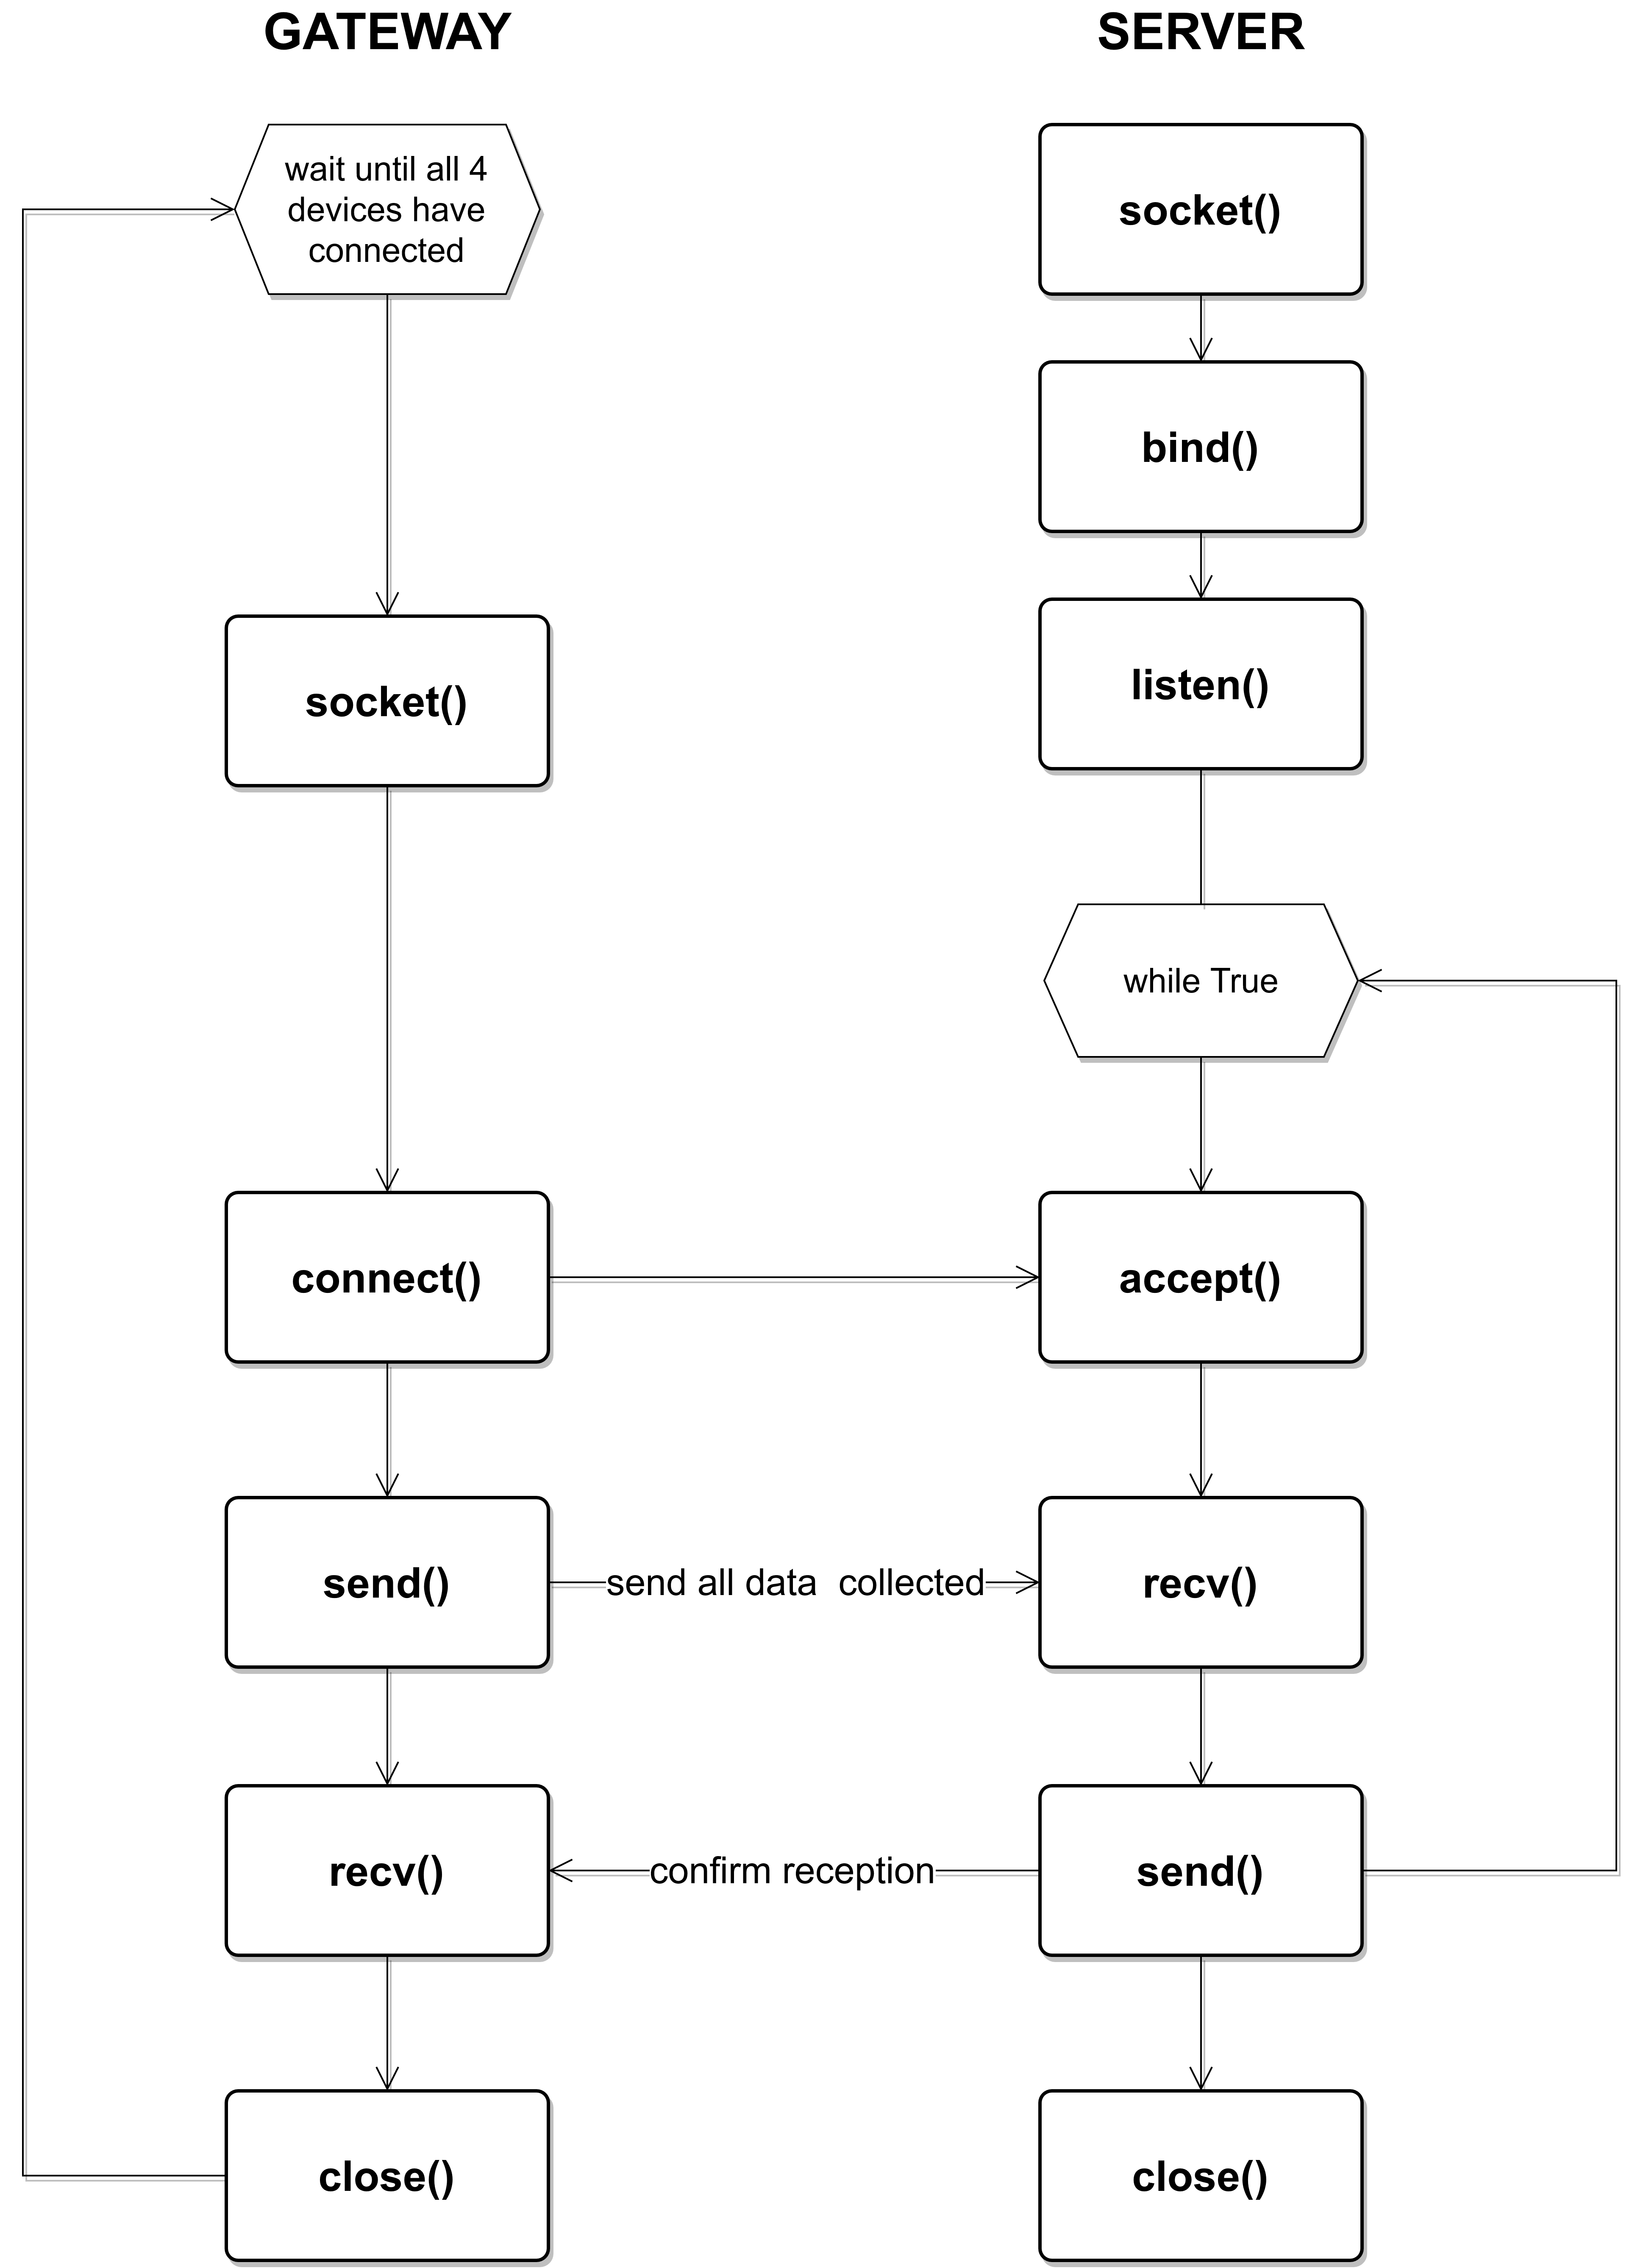
\includegraphics[scale=0.5]{UML/GatewayServer.png}
    \end{center}
    \caption{Schema rappresentante la comunicazione Gateway e Server}
    \label{img:GatewayServer}
\end{figure}
\section{Dimensione dei buffer}
\
\\
%
Per il dimensionamento dei buffer abbiamo tenuto conto del fatto che per una migliore corrispondenza con l'hardware e le realtà di rete, la dimensione del buffer in bytes dovrebbe essere una potenza relativamente piccola di 2. In fase di costruzione dell'architettura di rete abbiamo inoltre stimato le dimensioni dei pacchetti scambiati dalle diverse entità. Viste queste considerazioni ecco le dimensioni che abbiamo assegnato ai buffer di ricezione:
%
\begin{itemize}
    \item Per i \textbf{Device} in attesa di una risposta dal \textbf{DHCP} o dal \textbf{Gateway}, \texttt{1024 Bytes} risultano essere più che sufficienti;
    \item Per il \textbf{Gateway} in attesa di ricevere i dati dai device, tenuto conto che la dimensione di un pacchetto si aggira intorno ai \texttt{600-700 Bytes}, \texttt{1024 Bytes} sono sufficienti.
    \item Per il \textbf{Gateway} che attende la risposta da parte del \textbf{Server} \texttt{1024 Bytes} sono più che sufficienti;
    \item Per il \textbf{DHCP} che attende una richiesta di un \texttt{indirizzo IP}, \texttt{1024 Bytes} sono più che sufficienti.
    \item Per il \textbf{Server} che attende la ricezione delle misurazioni dei 4 dispositivi abbiamo assegnato una dimensione pari a \texttt{4096 Bytes} visto che la dimensione di un paccheto contente le misurazioni di \underline{un solo device} si aggira intorno ai \texttt{600 Bytes} (Considerati i 4 device, sono ca. 2400, da cui \texttt{4096 Bytes} per renderla una potenza di 2)
\end{itemize}


\chapter{Sviluppo}
\section{Metodologia di lavoro}
\subsection{GIT}
Lavorando in coppia abbiamo scelto di utilizzare \textit{Git} per condividere il lavoro ed il codice.\\
Nonostante pratici con \textit{branching} e \textit{GitFlow}, in questo caso non abbiamo ritenuto necessario il loro utilizzo.\\
\subsection{Visual Studio Live Share}
Abbiamo deciso in diverse occassioni di approcciarci allo sviluppo ed alle fasi di programmazione seguendo quello che è il pair-programming, grazie all'utilizzo dell'estensione \textit{Live Share} di \textit{Visual Studio}. Questo ci ha permesso di adottare uno stile ibrido e doubly-checked, prevenendo possibili errori oppure incomprensioni causate da un approccio asincrono.

\section{Note di sviluppo}
Per la formattazione dell'output abbiamo utilizzato una libreria di Python,
\texttt{beautifultable}, per la sua installazione basta lanciare il comand \texttt{pip install beautifultable}.\\
Per ulteriori informazioni si consulti \href{https://pypi.org/project/beautifultable/}{\underline{il seguente link}}.\\
Mentre per l'invio effettivo attraverso le socket dei "pacchetti" abbiamo optato per la serializzazione con l'utilizzo del modulo \href{https://docs.python.org/3/library/pickle.html}{\underline{pickle}}.
\appendix

\chapter{Guida utente}
Per testare efficacemente la simulazione è necessario seguire i seguenti step:
\begin{itemize}
    \item Lanciare il \texttt{Server} in un terminale dedicato con il comando:
        \begin{lstlisting}[language=bash]
            $ python IOT_server_TCP.py
        \end{lstlisting}
    \item Lanciare il \texttt{Gateway} in un terminale dedicato con il comando:
        \begin{lstlisting}[language=bash]
            $ python IOT_gateway.py
        \end{lstlisting}
    \item Lanciare i 4 \texttt{Device}, ciascuno in un terminale dedicato, con il comando:
        \begin{lstlisting}[language=bash]
            $ python IOT_device_UDP.py
        \end{lstlisting}
        assegnare poi a ciascun \texttt{Device} un proprio \textit{indirizzo MAC} quando richiesto da input.
\end{itemize}


\end{document}
